%
% 
%
\chapter{Resultados e Discussões} \label{chap:resultados}

\section{Avaliações Preliminares} \label{sec:avaliacoesespreliminares}

\subsection{Consistência dos Dados de Literatura}
\label{sec:dadosliteratura}

Após a implementação da metodologia descrita no \autoref{chap:metodologia}, os
resultados encontrados foram significativamente diferentes daqueles apresentados
por \citeonline{Rojas2014a}. A \autoref{fig:perfilTvalidacao}, por
exemplo, compara o perfil de temperatura dos leitos reais (de planta) com os
resultados da simulação implementada por \citeonline{Rojas2014a} e com os
resultados do trabalho aqui apresentado.

\begin{figure}[htb]
\centering 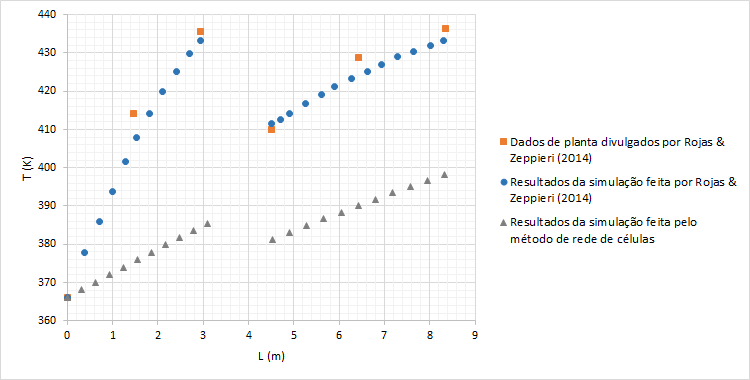
\includegraphics[scale=0.4]{images/Chap4/perfilTvalidacao.png}
\caption{Perfil de temperatura dos leitos.}
\label{fig:perfilTvalidacao}
\end{figure}

Duas questões precisam ser destacadas da \autoref{fig:perfilTvalidacao}.
A primeira delas refere-se a exortermia dos leitos catalíticos: a modelagem aqui
desenvolvida apresenta exortemia inferior aos demais dados. Esse fato, quando
analisado isoladamente, induz ao pensamento de que ou a simulação
por rede de células não fora bem equacionada ou a abordagem é inadequada para o
sistema estudado.

A segunda questão refere-se ao resfriamento na região zona de \emph{quench}. O
dado de planta apresenta um resfriamento de \SI{25,7}{K} entre os leitos
?? colocar este comando 'SI' para os outros valores no documento ??
catalíticos; a simulação de \citeonline{Rojas2014a} apresenta resfriamento de
$21,6 K$ para a região; e o valor encontrado no presente trabalho foi de $4,1
K$. Essa situação torna-se mais enigmática ao se constatar que o balanço de
energia proposto por \citeonline{Rojas2014a} para a região de \emph{quench}
contém simplificações não realizadas neste estudo.

Uma análise do valor de $LHSV$ (\emph{Liquid Hourly Space Velocity}) foi feita
na tentativa de trazer um esclarecimento às discrepâncias encontradas. O
parâmetro $LHSV$ pode ser definido como: 
\begin{equation}
LHSV = F_{vol}^L/{V_{R}}
\label{eq:LHSV}
\end{equation}
onde $F_{v}^L$ é a vazão volumétrica em \si{m^3/h} de líquido e $V_{R}$ é o
volume total do reator (somados os dois leitos).

\nomenclature{$F_v$}{Vazão volumétrica \nomunit{m^3/h}}
\nomenclature[S]{$v$}{Referente à volume}
\nomenclature{$V$}{Volume \nomunit{m^3}}
\nomenclature{$V_R$}{Volume total do reator \nomunit{m^3}}

A \autoref{tab:comparacaoLHSV} mostra alguns valores encontrados na literatura
para LHSV, incluindo o trabalho de \citeonline{Rojas2014a}.

\begin{table}[!htb]
\begin{center}
\caption{Comparação entre valores de $LHSV$ publicados na literatura}
\label{tab:comparacaoLHSV}
\small
\begin{tabular}{lccc}
{Autor} & {$F_v^L$($m^3/h$)} & {$V_R$ ($m^3$)} &
{LHSV ($1/h$)}
\\
\hline
{\citeonline{Arpornwichanop2008}} & $69$ & $60$ & $1,14$ \\
{\citeonline{Mederos2007}} & $165$ & $62$ & $2,66$ \\
{\citeonline{Rojas2014a}} & $347$ & $18$ & $19,76$ \\
\bottomrule
\end{tabular}
\end{center}
\end{table}

Comparativamente, fica claro que o valor de LHSV do trabalho de
\citeonline{Rojas2014a} está uma ordem de grandeza acima dos valores
comumente empregados nos projetos de reatores TBR.

Sendo assim, foi necessário ajustar o valor da vazão de alimentação de gasolina
de pirólise para que os dados apresentassem coerência. O critério
utilizado foi o grau de resfriamento que ocorre na região de \emph{quench}. De
maneira mais direta, a vazão foi modificata até que a diferença de temperatura entre
a saída do primeiro leito e entrada do segundo fossem semelhantes aos dados de
planta e, também, aos dados calculados por \citeonline{Rojas2014a}.

Após várias tentativas, o valor de $F_{w,1}$ foi alterado para $2,079.10^4
kg/h$. Com essa nova vazão, tanto o resfriamento da região de \emph{quench}
quando a exotermia dos leitos tornaram-se aderentes aos dados de planta e de
literatura, como está mostrado na \autoref{sec:estadoestacionario}.

A \autoref{tab:comparacaoLHSV2} repete os valores da
\autoref{tab:comparacaoLHSV}, mas agora com a inclusão do valor de LHSV
após o ajuste da vazão de carga do reator.

\begin{table}[!htb]
\begin{center}
\caption{Comparação entre LHSV}
\label{tab:comparacaoLHSV2}
\small
\begin{tabular}{lccc}
{Autor} & {$F_v^L$ ($m^3/h$)} & {$V_R$ ($m^3$)} &
{LHSV ($1/h$)}
\\
\hline
{\citeonline{Arpornwichanop2008}} & $69$ & $60$ & $1,14$ \\
{\citeonline{Mederos2007}} & $165$ & $62$ & $2,66$ \\
{\citeonline{Rojas2014a}} & $347$ & $18$ & $19,76$ \\
{Dados ajustados} & $76$ & $18$ & $4,34$ \\
\bottomrule
\end{tabular}
\end{center}
\end{table}

\subsection{Determinação do Valor de $N_{Disc}$} \label{sec:determinacaoNDisc}

Nesta seção será apresentado a maneira como foi escolhido o valor ideal de
$N_{Disc}$. O valor escolhido foi utilizado em todas as simulações doravante
apresentadas.

A maneira mais simples (e talvez a mais adequada) de se determinar o número de
células é simular o reator com diferentes valores de $N_{Disc}$ e, então,
comprá-los entre eles pelos resultados de variáveis chave. Duas variáveis foram
escolhidas: temperatura e fração molar global de hidrogênio.

O \autoref{fig:NDiscT} mostra o perfil de temperatura do leito superior, para
diferentes valores de $N_{Disc}$. Perceb-se que, para entre $N_{Disc} = 4$ e
$N_{Disc} = 8$ ainda há alguma diferença no comportamento do perfil de
temperatura. Contudo, é imperceptível a diferença entre os perfis resultantes de
$N_{Disc} = 8$ e $N_{Disc} = 16$. 

\begin{figure}[htb] \centering
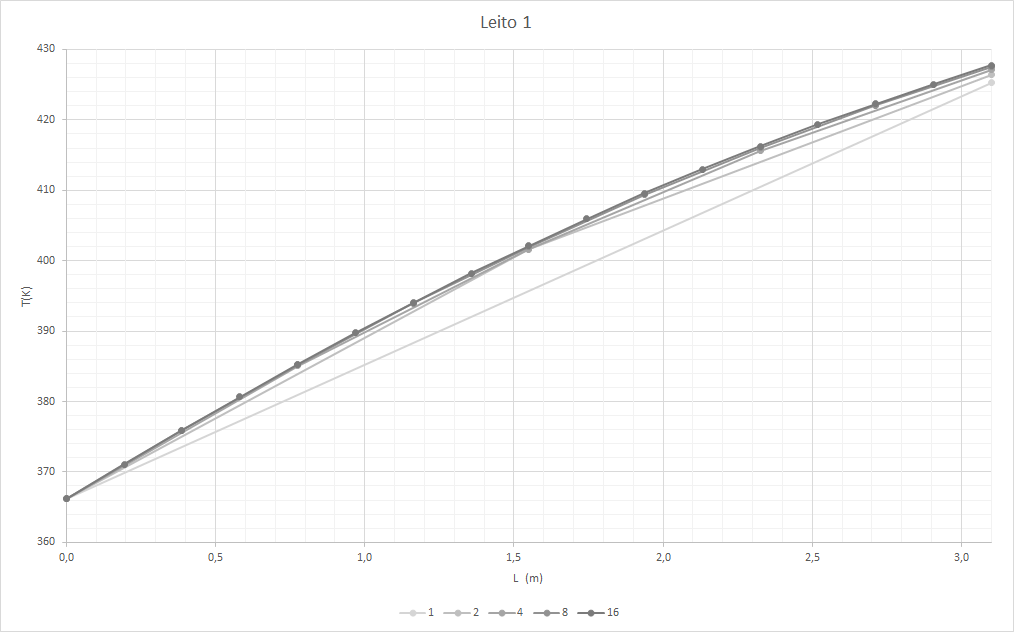
\includegraphics[scale=0.4]{images/Chap4/NDiscT.png}
\caption{Avaliação de NDisc pelo perfil de temperatura}
\label{fig:NDiscT}
\end{figure}

Observando o perfil da fração molar global de hidrogênio de diferentes valores
de $N_{Disc}$ (também para o leito superior), é ainda menos relevante a
diferença entre $N_{Disc} = 4$ e $N_{Disc} = 8$, como mostra a
\autoref{fig:NDiscz}.

\begin{figure}[htb]
\centering 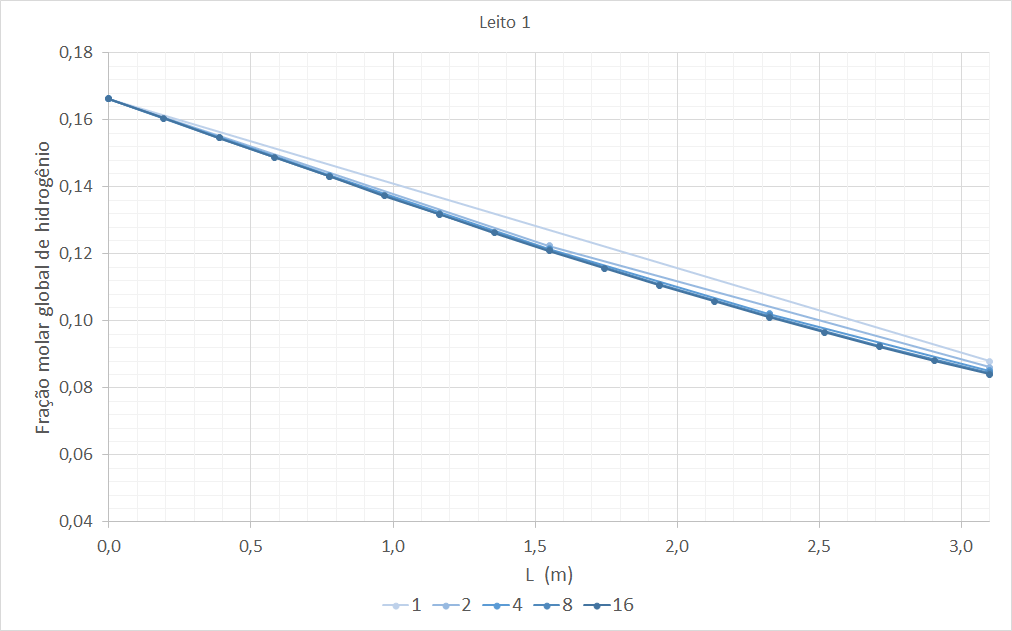
\includegraphics[scale=0.4]{images/Chap4/NDiscz.png}
\caption{Avaliação de NDisc pela fração molar total de hidrogênio}
\label{fig:NDiscz}
\end{figure}

Assim, discretizar cada leito catalítico em $8$ células pareceria uma escolha
razoável e suficiente para o objetivo deste trabalho. Entretanto, devido a
algumas questões de convergência do \emso, foi utilizado o valor de $N_{Disc} =
10$.

\subsection{Avaliação da Perda de Carga} \label{sec:avaliacaoperdadecarga}

A equação da perda de carga quando implementada no modelo do reator causou
alguns problemas de convergência. Assim, optou-se primeiramente por avaliar a
importância da perda de carga, e se ela alteraria muito o perfil de pressão a
ponto de inpactar no cálculo das propriedades das fases e do ELV.

Foi feita, portanto, uma simulação inicial que estimou a perda de carga, mas sem
alterar o perfil de pressão (pressão constante ao longo do reator). A perda de
carga estimada para os leitos está na \autoref{tab:perdadecarga}. Por esses
valores, percebe-se que a pressão ao longo dos leitos permanece praticamente
inalterada. Sendo assim, o reator foi simulado desprezando-se a perda de carga.

\begin{table}[!htb]
\begin{center}
\caption{Perda de Carga dos Leitos}
\label{tab:perdadecarga}
\small
\begin{tabular}{lccc}
{} & {$\Delta P/L$ ($atm/m$)} & {Pressão de entrada (atm)} & {Pressão de saída
(atm)}
\\
\hline
{Leito 1} & $3,4.10^{(-3)}$ & $49,64$ & $49,63$ \\
{Leito 2} & $3,7.10^{(-3)}$ & $49,63$ & $49,61$ \\
\bottomrule
\end{tabular}
\end{center}
\end{table}

Um valor tão baixo assim de perda de carga não é o comumente encontrado na
indústria. Porém, a equação utilizada por \citeonline{Rojas2014a} e aqui neste
trabalho pode não ser a mais adequada, já que houve uma alteração da vazão de
carga do reator. Está mostrado na \autoref{sec:estadoestacionario} que o regime
de escoamento do reator se altera de regime de bolha (alta interação),
considerado por \citeonline{Rojas2014a}, para regime de escoamento gotejante
(baixa interação). Assim, sendo, a equação para avaliação da perda de carga no
reator deveria ter sido outra mais adequada às características do sistema.

\section{Estado Estacionário} \label{sec:estadoestacionario}

\subsection{Perfil de Temperatura} \label{sec:perfildetemperatura}

A figura \autoref{fig:perfilT} mostra o perfil de temperatura dos leitos
calculado por este trabalho, além daquele calculado por \citeonline{Rojas2014a}
e pelos dados de planta por eles publicados.  

A diminuição drástica do valor da vazão de alimentação no reator aumenta o
valor do tempo de residência dos reagentes dentro do mesmo. Com mais tempo para
reagir, ocorre maior liberação de energia das reações de hidrogenação. O
interessante para o caso em questão é que o fato de haver uma vazão específica
que ajuste tanto o resfriamento na zona de \emph{quench} quanto o perfil de
temperatura.

\begin{figure}[htb]
\centering 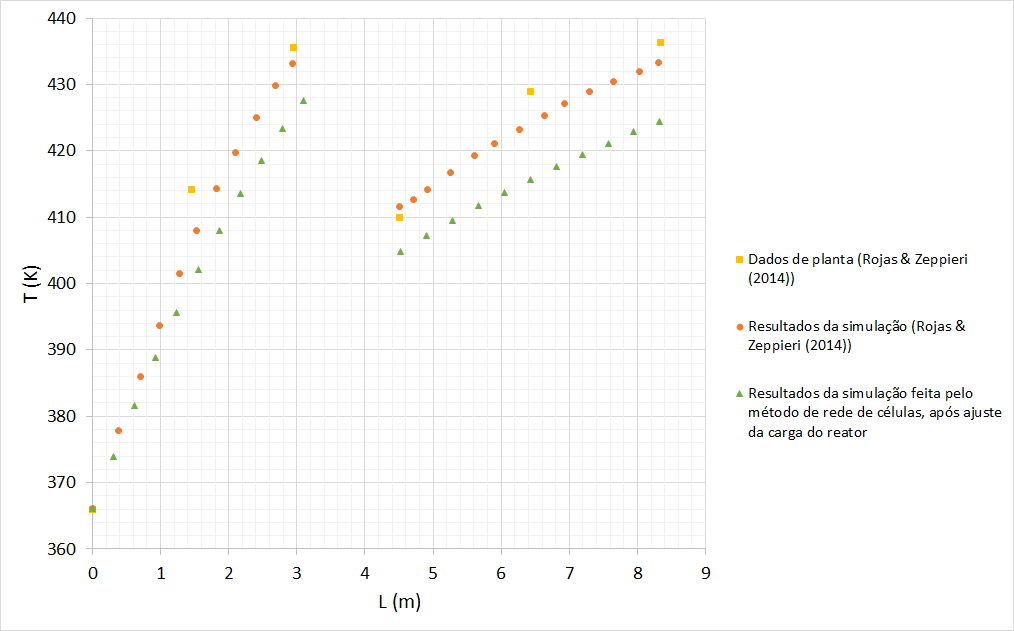
\includegraphics[scale=0.4]{images/Chap4/perfilT.png}
\caption{Perfil de temperatura dos leitos}
\label{fig:perfilT}
\end{figure}

\subsection{ELV}



\section{Respostas Dinâmicas} \label{sec:respostasdinamicas}





























